\documentclass[12pt,a4paper,oneside,ngerman]{article}
\usepackage[utf8]{inputenc}
\usepackage{color}
\usepackage{tikz}
\usepackage{amsmath}
\usepackage{amssymb}
\usepackage{calc}
\usepackage{mathtools}
\usepackage{float}
\usepackage{struktex}
\usepackage{ulem}

\title{EZS}
\author{Simon Krücken}

\begin{document}
    
%\begin{titlepage}
%    \maketitle
%\end{titlepage}
%\tableofcontents

\section[placeholder]{placeholder}
\section[Zentrale Beschreibgrößen]{Zentrale Beschreibgrößen}
\subsection{placeholder}

\paragraph[Defintion]{Defintion:}
Realzeitsystem haben neben Funktionalen Anforderungen auch \textcolor{red}{zeitliche} Anforderungen.

Ein Realzeitsystem besteht softwaretechnisch aus einer Reihe von Tasks und aus der System-Software.

\begin{figure}[ht]
	\centering
	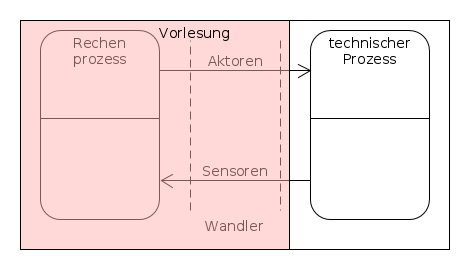
\includegraphics[scale=0.5]{umlet/rt_control.png}
\end{figure}

\subsubsection{Technischer Prozess}
Rechenzeitanforderung = Ereignis von technischen Prozess
Releasetime = Zeitpunkt des Auftretens der RZ-Anforderung (RZ/RT = Realzeit)

\paragraph[Beispiel]{Beispiel:}
periodisches Signal \textcolor{red}{u} alle 200ms

\fbox{
	\parbox{\textwidth}
	{
		\(t_{Release,u,1}\) = 0ms \(t_{Release,u,2}\) = 200ms \linebreak
		\(t_{Release,u,3}\) = 400ms \(t_{Release,u,4}\) = 600ms \linebreak
						
		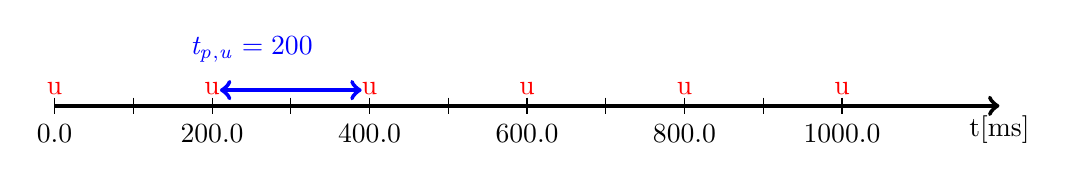
\begin{tikzpicture}
			\draw[ultra thick, ->] (0,0) -- (12,0);
			\draw[ultra thick, <->, draw=blue] (2.1,0.2) -- (3.9,0.2);
			\node[anchor=north] at (2.5,1) {\textcolor{blue}{\(t_{p,u} = 200\)}};
			\node[anchor=north] at (12,0) {t[ms]};
			\foreach \x in {0,1,2,3,4,5,6,7,8,9,10}
			\draw (\x cm,3pt) -- (\x cm,-3pt);
									
			\foreach \x in {0,2,4,6,8,10} {
				\pgfmathsetmacro\result{\x * 100}
				\draw[ultra thick] (\x,0) node[below=3pt,thick] {\result} node[above=3pt] {};
				\draw[ultra thick] (\x,0) node[above] {\textcolor{red}{u}} {};
			}
		\end{tikzpicture}
						
		\textcolor{blue}{Prozesszeit} = zeitlicher Abstand zwischen zwei \textcolor{red}{RZ-Anforderungen} gleichen Typs.
	}
}

\begin{quote}
    \(t_{Pmin,i} = minimal\) =$>$ \(t_{max,i} = \dfrac{1}{ t_{Pmin,i} }\) \\
	\(t_{Pmax,i} = maximal\) \textcolor{gray}{$<$= uninteressant} \\
	\(t_{Dmin,i}\) = minimal zulässige Reaktionszeit \\
	\(t_{Dmax,i}\) = maximal zulässige Reaktionszeit
\end{quote}

Airbag: \\
\(t_{Dmax}\) = 50ms(Zeit bis zum Aufschlag) - 30ms(Zeit zum aufblasen) = 20ms \\
\(t_{Dmin}\) = 0ms

Phase = minimal Zeitlicher Abstand zwischen zwei \textcolor{red}{unterschiedlicher} RZ-Anforderungen \(t_{Ph,i,j}\) \\

\subsubsection{Rechenprozesse}

\begin{description}
\item - Ausführuntgszeit (Executiontime) = Rechenzeit für eine RZ-Anforderung (ohne Warte oder Schlafzeiten)	
	\begin{description}
		\item - WCET \(t_{Emax,i}\) --$>$ Erfahrung oder Messen \textcolor{gray}{Worstcase}
		\item - BCET \(t_{Emin,i}\) = 0 \textcolor{gray}{Bestcase}
	\end{description}
\end{description}

\fbox{
	\parbox{\textwidth}
	{
		\textcolor{red}{ \(t_{E,u}\) = 100ms }
		\textcolor{blue}{ \(t_{E,t}\) = 50ms }
						
		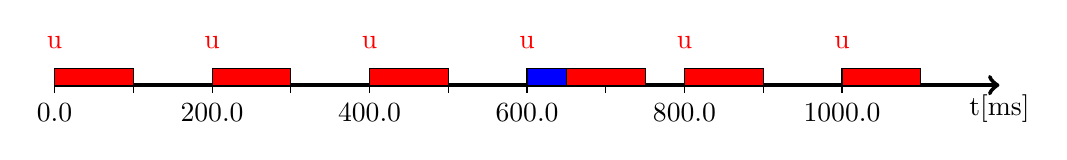
\begin{tikzpicture}
			\draw[ultra thick, ->] (0,0) -- (12,0);
			\node[anchor=north] at (12,0) {t[ms]};
			\foreach \x in {0,1,2,3,4,5,6,7,8,9,10}
			{
				\draw (\x cm,3pt) -- (\x cm,-3pt);
			}

			\foreach \x in {0,2,4,8,10}
			{
				\pgfmathsetmacro\result{\x+1}
				\draw [fill=red] (\x,0) rectangle (\result, 6pt);
			}
			
			\draw [fill=red] (6.5,0) rectangle (7.5, 6pt);
			\draw [fill=blue] (6,0) rectangle (6.5, 6pt);
									
			\foreach \x in {0,2,4,6,8,10} {
				\pgfmathsetmacro\result{\x * 100}
				\draw[ultra thick] (\x,0) node[below=3pt,thick] {\result} node[above=3pt] {};
				\draw[ultra thick] (\x,9pt) node[above] {\textcolor{red}{u}} {};
			}
		\end{tikzpicture}
	}
}

- Reaktionszeit \(t_{R,i}\) = Zeit zwischen den Auftreten der RZ-Anforderungen \textcolor{red}{i} und dem Ende der Bearbeitung. \\

\(T_{Rmax,i}\) = maximale Reaktionszeit \\
\(T_{Rmin,i}\) = minimale Reaktionszeit \\
\(T_{R,i}\) = \textcolor{red}{\(t_{W,i}\)} \(+ t_{E,i}\) wobei \textcolor{red}{ \(t_{W,i}\) } Summe aller Wartezeiten

\subsubsection{Systemsoftware}

- Latenzzeit \(t_{L_i}\) = Zeit zwischen dem Auftreten einer RZ-Anforderung und dem Start der Bearbeitung
\textcolor{blue}{
	- Interrup Latenzzeit
	- Tasklatenzzeit
}

\subsection{Realzeitbedingungen}
\subsubsection{Auslastungsbedingung}

\(\rho_i = \dfrac{t_{E,i}}{t_{P,i}}\) Auslastung dur RZ-Anforderung i \\

\(\rho_{max,i} = \dfrac{t_{Emax,i}}{t_{Pin,i}}\) Worstcase, max. Auslastung

\fbox{
	\parbox{\textwidth}
	{
		1. RT Bedingung

		\(\rho_{max,ges} = \displaystyle\sum_{j=1}^n \dfrac{t_{Emax,i}}{t_{Pin,i}} \leq c\) \\
		j = für alle RZ-Anforderungen,
		c = Anzahl der Rechnerkerne
	}
}

\fbox{
	\parbox{\textwidth}
	{
		Beispiel: 2 RZ-Anforderungen A und B

		\begin{equation*}
			\begin{rcases}
				t_{Pmin,A} &= 2ms \\
				t_{Emax,A} &= 0.8ms
			\end{rcases} 
			\text{\(\rho_{max,A} = \dfrac{0.8ms}{2ms} = 0.4ms \)}
		\end{equation*}

		\begin{equation*}
			\begin{rcases}
				t_{Pmin,B} &= 1ms \\
				t_{Emax,B} &= 0.3ms
			\end{rcases} 
			\text{\(\rho_{max,B} = \dfrac{0.3ms}{1ms} = 0.3ms \)}
		\end{equation*}

		\( \rho_{max,ges} = \rho_{max,A} + \rho_{max,B} = 0.7 = 70\% \) \\

		Annahme Singlecore c = 1
		\( \rho_{max,ges} \leq c \) =$>$ \textcolor{green}{\( 0.7 \leq 1\)}

		Auslastungsbedingung erfüllt
	}
}

\subsubsection{Rechtzeitigkeitsbedingung}
Für den Realzeitbetrieb muss die tatsächliche Reaktion innerhalb des Zulässigen Reaktionsbereiches erfolt sein.

\begin{figure}[ht]
	\centering
	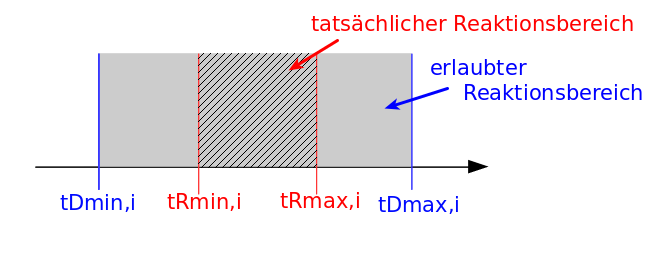
\includegraphics[scale=0.5]{umlet/Rechtzeitigkeitsbedingung.png}
\end{figure}

\fbox{
	\parbox{\textwidth}
	{
		2. RT Bedingung

		Für alle RZ-Anforderungen j muss gelten:

		\( t_{Dmin,j} \leq t_{Rmin,j} \leq t_{Rmax,j} \leq t_{Dmax,j} \)
	}
}

\subsubsection{Harte und weiche Realzeit}

\begin{figure}[H]
	\centering
	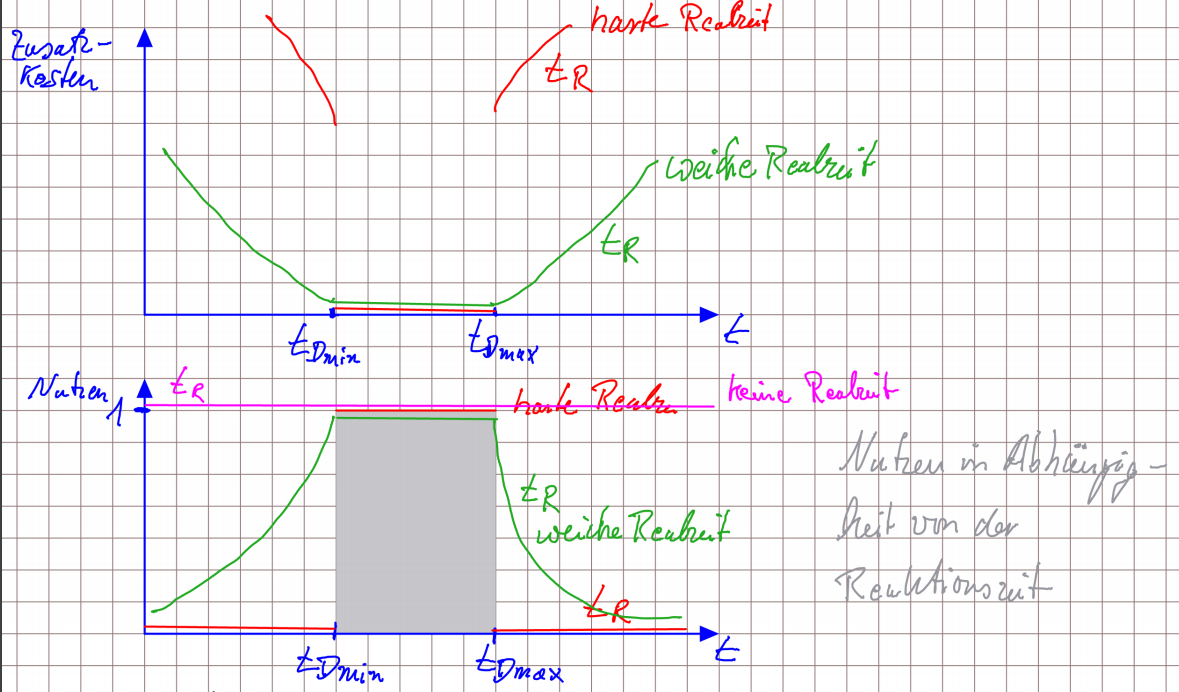
\includegraphics[scale=0.4]{umlet/harte_weiche_realzeit.png}
\end{figure}

\subsection{Systemaspekte}
\subsubsection{Unterbrechbarkeit}

\paragraph{Forderung:}
Codesequenzen lassen sich in Teilsequenzen unterteilen, die in Korrekter Reihenfolge aber unabhängig voneinander abgearbeitete werden können. \\
=$>$ notwendig für den Realzeitbetrieb

\paragraph{Begründung:}
Ein Messwert soll kontinuierlich erfasst werden. \\
\(t_{Emin,u} = t_{Emax,E} = 0.5ms\) \\
Jeweils 100 Messwerte (alle 100ms) sollen weiterverarbeitet werden \\
\(t_{Pmin,w} = 100ms\) \\
\(t_{Dmin,w} = 0ms\) \\
\(t_{Dmax,w} = 100ms\) \\
\(t_{Dmax,w} = 100ms\) \\ 
\(t_{Emin,w} = t_{Emax,w} = 40ms\) \\

Lösung (ohne Unterbrechbarkeit):\\
\begin{struktogramm}(95,40)
	\while[8]{while(1)}
		\while[7]{100 mal}
			\assign{Messwert einlese / \textcolor{green}{0.5ms}}
		\whileend
		\assign{weiterverarbeiten / \textcolor{green}{40ms}}
	\whileend
\end{struktogramm}

\fbox{
	\parbox{\textwidth}
	{					
		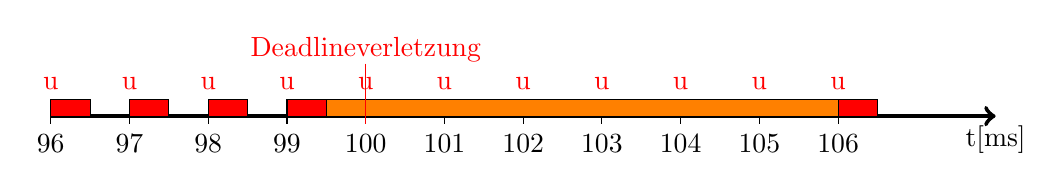
\begin{tikzpicture}
			\draw[ultra thick, ->] (0,0) -- (12,0);
			\node[anchor=north] at (12,0) {t[ms]};
			\foreach \x in {0,...,10}
			\draw (\x cm,3pt) -- (\x cm,-3pt);

			\foreach \x in {0,...,10}
			{
				\pgfmathsetmacro\result{\x+0.5}
				\draw [fill=red] (\x,0) rectangle (\result, 6pt);
			}
			
			\draw [fill=orange] (3.5,0) rectangle (10, 6pt);
			\draw [red](4,19pt) -- (4,-3pt);
			\draw [ultra thick] (4,0) node[above=16pt,thick] {\textcolor{red}{Deadlineverletzung}} {};

									
			\foreach \x in {96,...,106} {
				\pgfmathsetmacro\result{\x-96}
				\draw[ultra thick] (\result,0) node[below=3pt,thick] {\x} node[above=3pt] {};
				\draw[ultra thick] (\result,0) node[above=6pt,thick] {\textcolor{red}{u}} {};
			}
		\end{tikzpicture}
	}
}

\( \rho_{max,u} = \dfrac{0.5ms}{1ms} = 0.5 \);  \(\rho_{max} = \dfrac{40ms}{100ms} = 0.4\) =$>$  \(\rho_{max,ges} = 0.9 \)

Lösung mit Unterbrechbarkeit: \\

\begin{figure}[htb]
	\begin{minipage}[t]{0.4\textwidth}
		\begin{struktogramm}(50,35)
			\while[8]{while(1)}
				\while[7]{100 mal}
					\assign{Messwert einlese / \textcolor{green}{0.5ms}}
				\whileend
				\assign{Thread \textcolor{orange}{W} wecken}
			\whileend
			Thread \textcolor{red}{U}
		\end{struktogramm}%
	\end{minipage}%
	\hfill
	\begin{minipage}[t]{0.4\textwidth}
		\begin{struktogramm}(50,23)
			\while[8]{while(1)}
				\assign{schlafen}
				\assign{weiterverarbeiten}
			\whileend
			Thread \textcolor{orange}{W}
		\end{struktogramm}
	\end{minipage}
\end{figure}

\fbox{
	\parbox{\textwidth}
	{					
		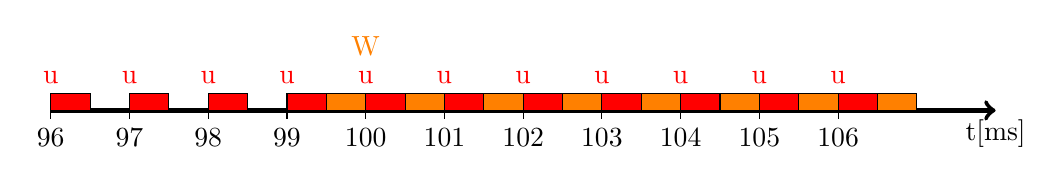
\begin{tikzpicture}
			\draw[ultra thick, ->] (0,0) -- (12,0);
			\node[anchor=north] at (12,0) {t[ms]};
			\foreach \x in {0,...,10}
			\draw (\x cm,3pt) -- (\x cm,-3pt);

			\foreach \x in {0,...,10}
			{
				\pgfmathsetmacro\result{\x+0.5}
				\draw [fill=red] (\x,0) rectangle (\result, 6pt);
			}

			\foreach \x in {3.5,...,10.5}
			{
				\pgfmathsetmacro\result{\x+0.5}
				\draw [fill=orange] (\x,0) rectangle (\result, 6pt);
			}
			
			\draw [ultra thick] (4,0) node[above=16pt,thick] {\textcolor{orange}{W}} {};
						
			\foreach \x in {96,...,106} {
				\pgfmathsetmacro\result{\x-96}
				\draw[ultra thick] (\result,0) node[below=3pt,thick] {\x} node[above=3pt] {};
				\draw[ultra thick] (\result,0) node[above=6pt,thick] {\textcolor{red}{u}} {};
			}
		\end{tikzpicture}
	}
}

\paragraph{Konsequenzen:}
\begin{description}
	\item a) Inter-prozess-Kommunikation (IPC) (Sync, Datenaustausch)
	\item b) Multithreading/Multitasking
\end{description}

\subsubsection{Prioritäten}
\paragraph{Forderung:}
Der Systemarchitekt muss einfluss auf die Abarbeitungsreihenfolge mehrerer Tasks nehmen können z.B. über Prioritäten.

\subsubsection{Ressourcenmanagment}
--$>$ später

\section[Systemsoftware]{Systemsoftware}
\subsection{Firmware}
\paragraph{Aufgabe:}
\begin{description}
	\item - Basisinitialisierung der Hardware
	\item - Diagnose
	\item - Betriebinitialisierung
	\item - Laden + Aktivieren von Codes
	\item - Runtime Services
\end{description}
\paragraph{Ausprägungen:}
\begin{description}
	\item - BIOS
	\item - UEFI
	\item - Bootloader ("\textcolor{green}{Das U-Boot}")
	\item - Monitor Software
\end{description}

\subsection{RT-OS}
\paragraph{Defintion.:}
Bezeichnung für alle Software-Komponenten, die
\begin{description}
	\item - die Ausführung der Applikationen und
	\item - die Verteilung der Betriebsmittel (Memory, Files, CPU, Drucker, ...) ermöglichen, steuern und überwachen.
\end{description}
\paragraph{Anforderungen:}
\begin{description}
	\item - Zeitverhalten
	\item - Ressourcenverbraucht
	\item - Zuverlässigkeit und Stabilität
	\item - Sicherheit
	\item - Flexibilität und Kompatibilität
	\item - Portierbarkeit
	\item - Skalierbarkeit
\end{description}
\paragraph{Beispiele:}
Sämtliche Betriebsysteme

\begin{figure}[H]
	\paragraph{Systemarchitektur}
	\centering
	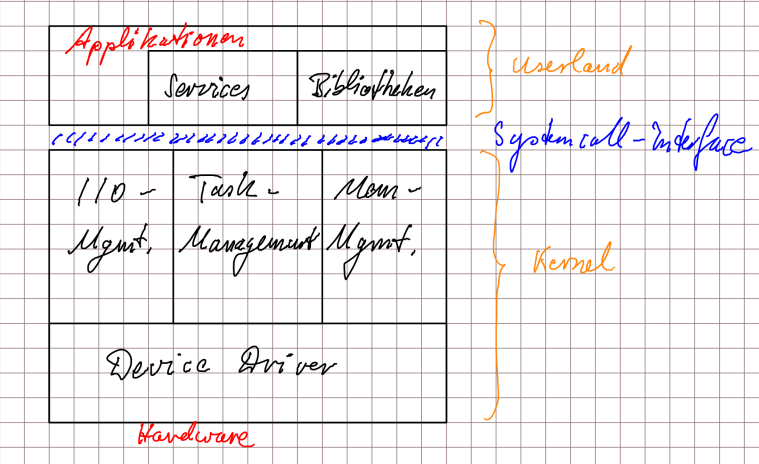
\includegraphics[scale=0.5]{umlet/systemarchitektur.png}
\end{figure}

\subsubsection{Systemcall-Interface}
Systemcall = Dienst des Kernels --$>$ 300-400 Dienste

\paragraph{Beispiele:}
open(), close(), read(), write(), exit(), fork(), clone(), clock\_nanosleep(), kill(), adjtime(),...\\
Technische Realisierung: SW-Interrupt

\paragraph{Ablauf:}
ret = write(fd, "Hello World", 13);\\
\textcolor{magenta}{ $\downarrow$ Systemcall "write" per SW-Interrupt}\\
\textcolor{magenta}{"int 0x80", "trap", "sysenter"}\\
\textcolor{magenta}{Systemcall mit EAR = 4} \textcolor{gray}{ $<$-- x86 Register} \\

\textcolor{blue}{ISR (SW-Interrupt 0x80) } \\
\textcolor{blue}{$\downarrow$ EAX = 4 --$>$ bedeutet write } \\
\textcolor{blue}{vfs\_write()} \\
\textcolor{blue}{$\downarrow$ wertet die übrigen CPU-Register aus } \\
\textcolor{blue}{$\downarrow$ fd --$>$ entscheidet über den zu nutzenden Gerätetreiber } \\
\textcolor{blue}{driver\_write() --$>$ gibt Hardwaretehcnisch die Daten aus} \\

\subsubsection{Taskmanagment}
\paragraph{Aufgabe:}
Verwaltung der Ressource CPU
\begin{description}
	\item --$>$ quasi parallele Verarbeitung auf einzelenen CPU-Kernen
	\item --$>$ real parallele Verarbeitung auf Multicore-Rechnern
\end{description}
Scheduling = Auswahl des als nächsten zu bearbeiten Jobs \\
Content Switch = Aktivierung eines Jobs \\

\paragraph{Singelcore-Scheduling}
Realisierung: Modifikation der Rücksprungadresse auf dem Stack beim Interrupt.

\begin{figure}[htbp]
	\begin{minipage}[t]{6cm}
	\vspace{0pt}
	\centering
	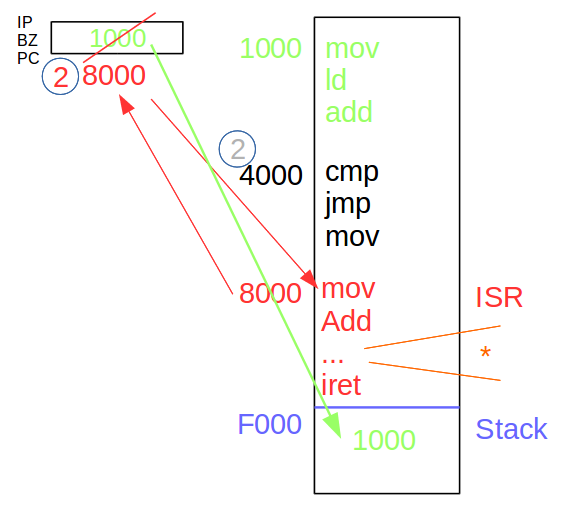
\includegraphics[scale=0.35]{umlet/Singelcore_scheduling.png}
	\end{minipage}
	\hfill
	\begin{minipage}[t]{6cm}
	\vspace{0pt}
	\begin{description}
	\item 1. \textcolor{blue}{Code an der im IP stehenen Address wird abgearbeitete}
	\item 2. \textcolor{blue}{IR tritt auf}
		\begin{description}
			\item - Inhalt vom IP wird auf den Stack gelegt
			\item - IP wird auf die Addresse der ISR gelegt (CPU arbeitet die ISR ab)
		\end{description}
	\item 3. \textcolor{blue}{Bei } \textcolor{red}{iret} \textcolor{blue}{ wird die auf dem stack hinterlegte Addresse zurück auf den IP geladen}
	\item --$>$ normale Verarbeitung wird fortgesetzt
	\end{description}
	\end{minipage}

	\textcolor{orange}{* zusätlicher Code der die auf dem Stack liegende Adresse ändert} \\
	\textcolor{orange}{z.B. die} \textcolor{green}{1000} \textcolor{orange} {wird mit} 4000 \textcolor{orange}{überschrieben} \\
\end{figure}





\end{document}